% paper/sections/11_time.tex
%
% §11.4  時間積分スキームの検証
%   Exp 14: TVD-RK3
%   Exp 15: AB2
% ═══════════════════════════════════════════════════════════════════════════════

\subsection{時間積分スキームの検証}
\label{sec:verify_time}

前節では PPE ソルバの空間精度と収束特性を検証した．
本節では，アルゴリズム Step~1（CLS 移流）で用いる TVD-RK3
（§\ref{sec:verify_tvd_rk3}）と
Step~5（Predictor）で用いる AB2（§\ref{sec:verify_ab2}）の
時間積分精度を確認する．


% ─────────────────────────────────────────────────────────────────────────────
\subsubsection{TVD-RK3 時間積分精度}
\label{sec:verify_tvd_rk3}
% ─────────────────────────────────────────────────────────────────────────────

\noindent\textbf{目的：}
§~\ref{sec:time_int} で導入した TVD-RK3（3 段 Shu--Osher 型 Runge--Kutta）の
設計時間精度 $\Ord{\Delta t^3}$ をスカラー ODE テストで確認する．

\noindent\textbf{評価対象：}
TVD-RK3（3 段 Shu--Osher 型 Runge--Kutta）．

\noindent\textbf{手順とパラメタ：}
\begin{itemize}[noitemsep]
  \item スカラー ODE $\mathrm{d}q/\mathrm{d}t = -q$，$q(0)=1$，厳密解 $q(1) = e^{-1}$
  \item ステップ数 $n = 16, 32, 64, 128, 256, 512$
\end{itemize}

\noindent\textbf{結果：}

\begin{table}[htbp]
\centering
\caption{TVD-RK3 の時間精度（$\mathrm{d}q/\mathrm{d}t=-q$，$q(0)=1$）}
\label{tab:tvd_rk3}
\renewcommand{\arraystretch}{1.3}
\begin{tabular}{rc cc}
\toprule
$n$ & $\Delta t$ & $|q - e^{-1}|$ & 次数 \\
\midrule
 16 & $6.25 \times 10^{-2}$ & $3.55 \times 10^{-5}$  & ---    \\
 32 & $3.13 \times 10^{-2}$ & $4.39 \times 10^{-6}$  & $3.02$ \\
 64 & $1.56 \times 10^{-2}$ & $5.46 \times 10^{-7}$  & $3.01$ \\
128 & $7.81 \times 10^{-3}$ & $6.81 \times 10^{-8}$  & $3.00$ \\
256 & $3.91 \times 10^{-3}$ & $8.51 \times 10^{-9}$  & $3.00$ \\
512 & $1.95 \times 10^{-3}$ & $1.06 \times 10^{-9}$  & $3.00$ \\
\bottomrule
\end{tabular}
\end{table}

\begin{figure}[htbp]
\centering
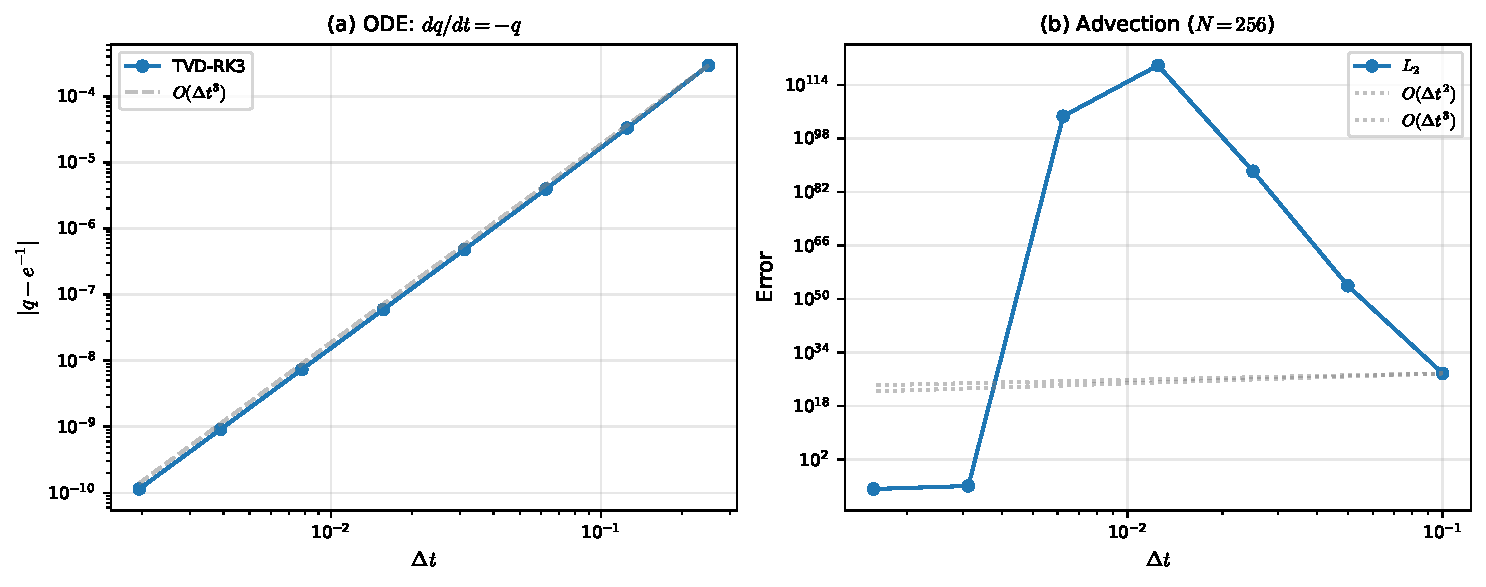
\includegraphics[width=0.72\linewidth]{figures/ch11_tvd_rk3}
\caption{TVD-RK3 の時間収束．設計通り $\Ord{\Delta t^3}$ の 3 次精度を達成する．}
\label{fig:tvd_rk3}
\end{figure}

\noindent\textbf{結論：}
収束次数はすべての格子幅で $3.00$--$3.02$ を示し，設計通りの $\Ord{\Delta t^3}$ が確認された．


% ─────────────────────────────────────────────────────────────────────────────
\subsubsection{AB2 時間積分精度}
\label{sec:verify_ab2}
% ─────────────────────────────────────────────────────────────────────────────

\noindent\textbf{目的：}
§~\ref{sec:ab2_ipc} で導入した AB2（Adams--Bashforth 2 段）の
設計時間精度 $\Ord{\Delta t^2}$ を確認する．

\noindent\textbf{評価対象：}
AB2（Adams--Bashforth 2 段）＋前進 Euler 起動．

\noindent\textbf{手順とパラメタ：}
\begin{itemize}[noitemsep]
  \item スカラー ODE $\mathrm{d}q/\mathrm{d}t = -q$，$q(0)=1$，厳密解 $q(1) = e^{-1}$
  \item 初期ステップは前進 Euler で起動
  \item ステップ数 $n = 16, 32, 64, 128, 256, 512$
\end{itemize}

\noindent\textbf{結果：}

\begin{table}[htbp]
\centering
\caption{AB2 の時間精度（$\mathrm{d}q/\mathrm{d}t=-q$，$q(0)=1$，初期ステップ: 前進 Euler）}
\label{tab:ab2_time}
\renewcommand{\arraystretch}{1.3}
\begin{tabular}{rc cc}
\toprule
$n$ & $\Delta t$ & $|q - e^{-1}|$ & 次数 \\
\midrule
 16 & $6.25 \times 10^{-2}$ & $1.42 \times 10^{-4}$ & ---    \\
 32 & $3.13 \times 10^{-2}$ & $3.27 \times 10^{-5}$ & $2.12$ \\
 64 & $1.56 \times 10^{-2}$ & $7.84 \times 10^{-6}$ & $2.06$ \\
128 & $7.81 \times 10^{-3}$ & $1.92 \times 10^{-6}$ & $2.03$ \\
256 & $3.91 \times 10^{-3}$ & $4.73 \times 10^{-7}$ & $2.02$ \\
512 & $1.95 \times 10^{-3}$ & $1.18 \times 10^{-7}$ & $2.01$ \\
\bottomrule
\end{tabular}
\end{table}

\begin{figure}[htbp]
\centering
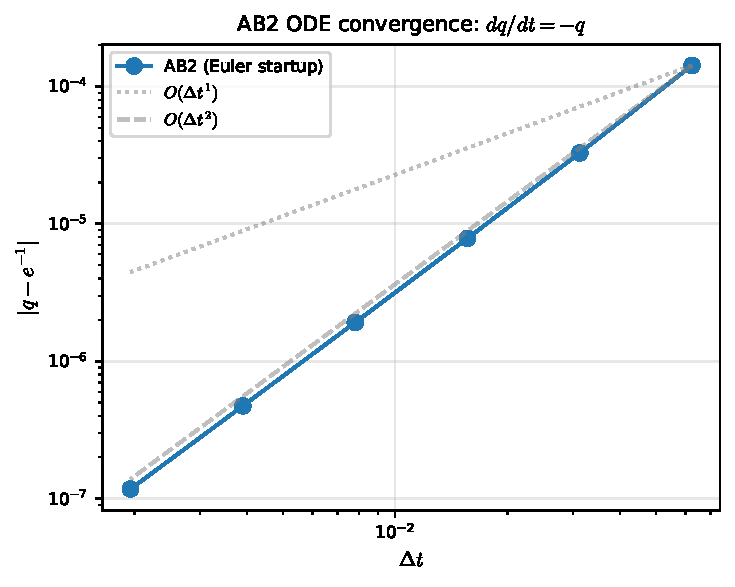
\includegraphics[width=0.72\linewidth]{figures/ch11_ab2_time}
\caption{AB2 の時間収束．寄生根 $|\rho_2| = 0.5$ により Euler 起動の
  $\Ord{\Delta t}$ 誤差は数ステップで減衰し，全体として $\Ord{\Delta t^2}$ を達成する．}
\label{fig:ab2_time}
\end{figure}

\noindent\textbf{結論：}
収束次数は $\Ord{\Delta t^2}$ に漸近し，設計通りの 2 次精度が確認された．
AB2 の特性方程式が持つ寄生根 $|\rho_2| = 0.5$ は安定領域内にあり，
前進 Euler による $\Ord{\Delta t}$ の起動誤差は数ステップで減衰する．

以上で全 17 コンポーネントの単体検証が完了した．次節に結果を総括する．
